\section{Bedrock model identifiers and pricing}
\label{app:models}

All LLM-agent experiments run against AWS Bedrock. Anthropic
models use the native tool-use API; the other four vendors use the
unified Bedrock Converse API through a thin adapter, so the agent
loop is identical across vendors. Table~\ref{tab:bedrock} lists
exact identifiers and per-token pricing used for all cost figures.

\begin{table*}[t]
\centering
\small
\begin{tabular}{llll}
\toprule
\textbf{Label} & \textbf{Vendor} & \textbf{Bedrock identifier} & \textbf{Pricing (per 1M tok, in/out)} \\
\midrule
Haiku~4.5     & Anthropic & \texttt{us.anthropic.claude-haiku-4-5-20251001-v1:0}  & \$1.00 / \$5.00 \\
Sonnet~4.5    & Anthropic & \texttt{us.anthropic.claude-sonnet-4-5-20250929-v1:0} & \$3.00 / \$15.00 \\
Sonnet~4.6    & Anthropic & \texttt{us.anthropic.claude-sonnet-4-6}               & \$3.00 / \$15.00 \\
Opus~4.8      & Anthropic & \texttt{us.anthropic.claude-opus-4-8}                 & \$5.00 / \$25.00 \\
Nova~Pro      & Amazon    & \texttt{amazon.nova-pro-v1:0}                         & \$0.80 / \$3.20 \\
DeepSeek~V3.2 & DeepSeek  & \texttt{deepseek.v3.2}                                & \$0.27 / \$1.10 \\
Ministral~8B  & Mistral   & \texttt{mistral.ministral-3-8b-instruct}             & \$0.10 / \$0.10 \\
Qwen3~32B     & Alibaba   & \texttt{qwen.qwen3-32b-v1:0}                          & \$0.15 / \$0.60 \\
\bottomrule
\end{tabular}
\caption{The eight Bedrock models (five vendors) and their
per-token list pricing as of May 2026, used for all cost figures in
the paper.}
\label{tab:bedrock}
\end{table*}

Across the leaderboard runs of
\S\ref{sec:cap-portability} (seven models, using and synthesizing
conditions), the agents consumed 25.4M input and 882k output tokens in total;
per-configuration token counts are stored in each result JSON.
The synthesis pipeline (\S\ref{sec:onboarding}) uses Sonnet~4.5 as
its default agent. The cross-model capability study
(\S\ref{sec:cap-portability}) sweeps all seven of the other models
above on the full 13-task SO-101 suite; smaller open-weight models
(Ministral~8B, Qwen3~32B) and a strong open model (DeepSeek~V3.2)
are included to test whether synthesis is restricted to the
strongest closed models.
Gemma-3 and Llama-3/4 were excluded after a tool-use smoke test:
Gemma-3-27B does not emit Converse tool calls, and the Llama
endpoints required an inference profile not available in our
account.

Figure~\ref{fig:cost-quality} combines this pricing with the
\S\ref{sec:cap-portability} leaderboard into a single cost--quality
plane: each point is one model $\times$ method configuration over
the full 13-task suite at $N{=}5$.

\begin{figure}[t]
\centering
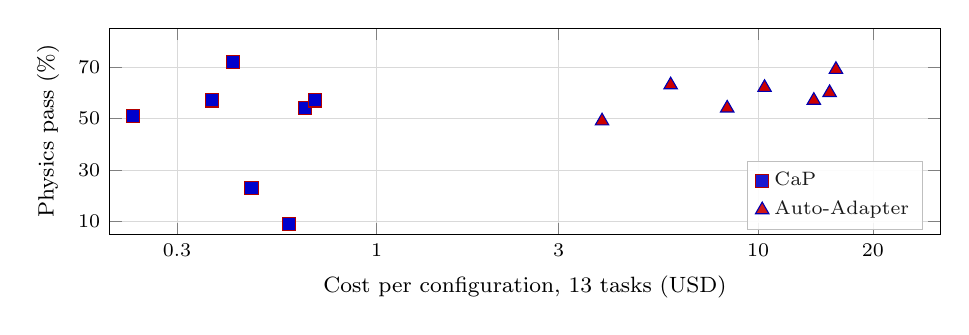
\begin{tikzpicture}
\begin{axis}[
  width=\columnwidth,
  height=4.2cm,
  xmode=log,
  log basis x=10,
  xlabel={\footnotesize Cost per configuration, 13 tasks (USD)},
  ylabel={\footnotesize Physics pass (\%)},
  xmin=0.2, xmax=30,
  ymin=5, ymax=85,
  xtick={0.3,1,3,10,20},
  xticklabels={0.3,1,3,10,20},
  ytick={10,30,50,70},
  grid=both,
  major grid style={line width=0.1pt, draw=gray!30},
  minor grid style={line width=0.05pt, draw=gray!15},
  tick label style={font=\scriptsize},
  legend style={font=\scriptsize, at={(0.98,0.02)}, anchor=south east,
                draw=gray!50, fill=white, fill opacity=0.9},
  legend cell align={left},
]
% CaP series (cost, phys): 7 models
\addplot+[only marks, mark=square*, mark size=2.4pt,
          draw=red!70!black, fill=red!40]
  coordinates {(0.65,54) (0.69,57) (0.23,51) (0.37,57) (0.59,9) (0.47,23) (0.42,72)};
\addlegendentry{CaP}
% Auto-Adapter series (cost, phys): 7 models
\addplot+[only marks, mark=triangle*, mark size=2.8pt,
          draw=blue!70!black, fill=blue!40]
  coordinates {(10.4,62) (16.0,69) (5.9,63) (15.4,60) (14.0,57) (8.3,54) (3.9,49)};
\addlegendentry{Auto-Adapter}
\end{axis}
\end{tikzpicture}
\caption{Cost--quality on the full 13-task SO-101 suite, seven
models $\times$ two methods (\S\ref{sec:cap-portability}).
Triangles (ours) occupy a higher-success, higher-cost regime;
squares (CaP) are cheap but high-variance (the high CaP outlier is
Qwen3~32B). Cost is per 13-task configuration at $N{=}5$.}
\label{fig:cost-quality}
\end{figure}

